\documentclass[conference]{IEEEtran}
\IEEEoverridecommandlockouts
% The preceding line is only needed to identify funding in the first footnote. If that is unneeded, please comment it out.
\usepackage{cite}
\usepackage{amsmath,amssymb,amsfonts}
\usepackage{algorithmic}
\usepackage{graphicx}
\usepackage{stfloats}
\usepackage{textcomp}
\usepackage{xcolor}
\usepackage{balance}
\usepackage{weiwAlgorithm}
\usepackage{xspace}
\usepackage{url}
\usepackage{subcaption}
\usepackage{authblk}

\captionsetup{compatibility=false}

%\newcommand\red[1]{\color{red}#1}
%\renewcommand\red[1]{#1}

%\renewcommand{\baselinestretch}{0.97}

\sloppy
%\newcounter{example}[section]
%\renewcommand{\theexample}{\nthesection.\arabic{example}}
%\newenvironment{example}{
%     \refstepcounter{example}
%     {\vspace{1ex} \noindent\bf  Example  \theexample:}}{
%     \eop\vspace{1ex}} %\hspace*{\fill}\vspace*{1ex}}

%\newcounter{definition}[section]
%\renewcommand{\thedefinition}{\nthesection.\arabic{definition}}
%\newenvironment{definition}{
%     \refstepcounter{definition}
%     {\vspace{1ex} \noindent\bf  Definition  \thedefinition:}}{
%     \eop\vspace{1ex}} %\hspace*{\fill}\vspace*{1ex}}

%\newcounter{theorem}[section]
%\renewcommand{\thetheorem}{\nthesection.\arabic{theorem}}
%\newenvironment{theorem}{\begin{em}
%         \refstepcounter{theorem}
%         {\vspace{1ex} \noindent\bf  Theorem  \thetheorem:}}{
%         \end{em}\eop\vspace{1ex}} %\hspace*{\fill}\vspace*{1ex}}
%
% \newcounter{lemma}[section]
% \renewcommand{\thelemma}{\nthesection.\arabic{lemma}}
% \newenvironment{lemma}{\begin{em}
%         \refstepcounter{lemma}
%         {\vspace{1ex}\noindent\bf Lemma \thelemma:}}{
%         \end{em}\eop\vspace{1ex}} %\hspace*{\fill}\vspace*{1ex}}
%
% \newcounter{remark}[section]
% \renewcommand{\theremark}{\nthesection.\arabic{remark}}
% \newenvironment{remark}{\begin{em}
%         \refstepcounter{remark}
%         {\vspace{1ex}\noindent\bf Remark \theremark:}}{
%         \end{em}\eop\vspace{1ex}} %\hspace*{\fill}\vspace*{1ex}}
%
% \newcounter{corollary}[section]
% \renewcommand{\thecorollary}{\nthesection.\arabic{corollary}}
% \newenvironment{corollary}{\begin{em}
%         \refstepcounter{corollary}
%         {\vspace{1ex}\noindent\bf Corollary \thecorollary:}}{
%         \end{em}\eop\vspace{1ex}} %\hspace*{\fill}\vspace*{1ex}}


\newcommand{\proofsketch}{\noindent{\bf Proof Sketch: }}
\newcommand{\myproof}{\noindent{\bf Proof: }}
% \newcommand{\proof}{\noindent{\em Proof: }}

\newcommand{\nthesection}{\arabic{section}}
% \newcommand{\thetheorem}{\thesection.\arabic{theorem}}


% End of proof
\newcommand{\eop}{\hspace*{\fill}\mbox{$\Box$}}
% \renewcommand{\eop}{\hspace*{\fill}\mbox{$\Box$}\vspace*{1ex}}

% Small Title
\newcommand{\stitle}[1]{\vspace{1ex} \noindent{{\bf #1}}}

\newcommand{\sstitle}[1]{\vspace{1ex} \noindent{\textit{ #1}}}
\newcommand{\ssstitle}[1]{\vspace{1ex} \noindent{\textbf{ #1}}}

\newcommand{\kw}[1]{{\ensuremath {\mathsf{#1}}}\xspace}
\newcommand{\bkw}[1]{{\ensuremath {\mathsf{\textbf{#1}}}}\xspace}

\newcommand{\kwnospace}[1]{{\ensuremath {\mathsf{#1}}}}
\newcommand{\ltt}{\kw{LTT}}
\newcommand{\arr}{\kw{arrive}}
\newcommand{\vp}{\kw{p}}

\newcommand{\bellf}{{\sc Bellman-Ford}\xspace}
\newcommand{\bfalgo}{{\sc OR}\xspace}

\newcommand{\aalgo}{{\sc KDXZ}\xspace}

\newcommand{\dijk}{{\sc Dijkstra}\xspace}
%\newcommand{\dalgo}{{\sc DLY}\xspace}
\newcommand{\dalgo}{{\sc Two-Step-LTT}\xspace}

\newcommand{\dtalgo}{{\sc DOT}\xspace}


\newcommand{\genfunc}{{\sl timeRefinement}\xspace}
\newcommand{\pathc}{{\sl pathSelection}\xspace}
\newcommand{\fifo}{{\sl FIFO}\xspace}

\newcommand{\st}{starting time\xspace}
\newcommand{\sti}{starting-time interval\xspace}
\newcommand{\stsi}{starting-time subinterval\xspace}
\newcommand{\stsis}{starting-time subintervals\xspace}
\newcommand{\stis}{starting-time intervals\xspace}
\newcommand{\ti}{time interval\xspace}
\newcommand{\tis}{time intervals\xspace}
\newcommand{\ttime}{travel time\xspace}
\newcommand{\ttimea}{travel time\xspace}
\newcommand{\at}{arrival time\xspace}
\newcommand{\ata}{arrival-time\xspace}
\newcommand{\atf}{arrival-time function\xspace}
\newcommand{\ati}{arrival-time interval\xspace}
\newcommand{\ats}{arrival times\xspace}
\newcommand{\ed}{edge delay\xspace}
\newcommand{\eda}{edge-delay\xspace}
\newcommand{\edf}{edge-delay function\xspace}
\newcommand{\eds}{edge delays\xspace}
\newcommand{\wt}{waiting time\xspace}

\newcommand{\g}{\overline{g}}
\newcommand{\iend}{\tau}

\newcommand{\argmin}{\operatornamewithlimits{argmin}}


%%%%%%%%%%%%%%%%%%%%%%%%%%%%%%%%%%%%%%%%%% Defined in XML Paper %%%%%%%%%%%%%%%%%%%%%%%%%%%%%%%%%%%%%%%%%%%%%%
\newcommand{\myhead}[1]{\vspace{.05in} \noindent {\bf #1.}~~}
\newcommand{\cond}[1]{(\emph{#1})~}
\newcommand{\op}[1]{(\emph{#1})~}

\newcommand{\qc}{\ensuremath{Q^c}}


\newcommand{\rewrite}{\kw{XPathToReg}}

\newcommand{\upparen}[1]{\ensuremath{\mathrm{(}}{#1}\ensuremath{\mathrm{)}}}
\newcommand{\func}[2]{\funcname{#1}\upparen{\ensuremath{#2}}}
\newcommand{\funcname}[1]{\ensuremath{\mathit{#1}}}

\newcommand\AS{\textbf{as}\ }
\newcommand{\xsltsize}{\small}

\newcommand{\X}{{\cal X}}
%\newcommand{\U}{{\cal U}}
\newcommand{\sem}[1]{[\![#1]\!]}
\newcommand{\NN}[2]{#1\sem{#2}}
\newcommand{\pcdata}{{\tt str}\xspace}

\newcommand{\exa}[2]{{\tt\begin{tabbing}\hspace{#1}\=\hspace{#1}\=\+\kill #2\end{tabbing}}}
\newcommand{\ra}{\rightarrow}
\newcommand{\la}{\leftarrow}
\newcommand{\rsa}{\_} % {\rightsquigarrow}
\newcommand{\Ed}[2]{E_{{\scriptsize \mbox{#1} \rsa \mbox{#2}}}}
\newenvironment{bi}{\begin{itemize}
        \setlength{\topsep}{0.5ex}\setlength{\itemsep}{0ex}\vspace{-0.6ex}}
        {\end{itemize}\vspace{-1ex}}
\newenvironment{be}{\begin{enumerate}
        \setlength{\topsep}{0.5ex}\setlength{\itemsep}{0ex}\vspace{-0.6ex}}
        {\end{itemize}\vspace{-1ex}}
\newcommand{\ei}{\end{itemize}}
\newcommand{\ee}{\end{enumerate}}

\newcommand{\mat}[2]{{\begin{tabbing}\hspace{#1}\=\+\kill #2\end{tabbing}}}
\newcommand{\m}{\hspace{0.05in}}
\newcommand{\ls}{\hspace{0.1in}}
\newcommand{\beqn}{\begin{eqnarray*}}
\newcommand{\eeqn}{\end{eqnarray*}}

\newcounter{ccc}
\newcommand{\bcc}{\setcounter{ccc}{1}\theccc.}
\newcommand{\icc}{\addtocounter{ccc}{1}\theccc.}

\newcommand{\oneurl}[1]{\texttt{#1}}
\newcommand{\tabstrut}{\rule{0pt}{4pt}\vspace{-0.1in}}
\newcommand{\tabstruct}{\rule{0pt}{8pt}\\[-2ex]}
\newcommand{\stab}{\rule{0pt}{8pt}\\[-2.2ex]}
\newcommand{\sstab}{\rule{0pt}{8pt}\\[-2.2ex]}

\newcommand{\eat}[1]{}

% \newfloat{tcm}{thp}{loa}
% \floatname{tcm}{Recursive \sql}

\def\subfigcapskip{2pt}
% \def\subfigtopskip{0pt}
% \def\subfigbottomskip{0pt}

%%%%%%%%%%%%%%%%%%%%%%%%%%%%%%%%%%%%%%%%%% Defined in XML Paper (END) %%%%%%%%%%%%%%%%%%%%%%%%%%%%%%%%%%%%%%%%%%%%%%

\newcommand{\rdms}{{\sc rdbms}\xspace}
\newcommand{\sql}{{\sc sql}\xspace}
\newcommand{\dbms}{{\sc dbms}\xspace}

%\newcommand{\cfig}{Figure~}
%\newcommand{\ctab}{Table~}
\newcommand{\cfig}{Fig.~}
\newcommand{\ctab}{Table~}
\newcommand{\csec}{Section~}
\newcommand{\cdef}{Definition~}
\newcommand{\cthm}{Theorem~}
\newcommand{\clem}{Lemma~}
\newcommand{\cequ}[1]{Equation~(#1)}
\newcommand{\SG}{\mathbf{SG}}
\newcommand{\SA}{\mathbf{SA}}
\renewcommand{\AA}{\mathbf{AA}}

%\newcommand{\EDA}{\textbf{EDA}}
%\newcommand{\CSP}{\textbf{CSP}}
%\newcommand{\TDSP}{\textbf{TDSP}}
%\newcommand{\SSSP}{\textbf{SSSP}}

%\newcommand{\revised}{***\texttt}
%\newcommand{\revised}{\comment}
%\newcommand{\add}{***{\texttt{ADD}}}
%\newcommand{\add}{}
%\newcommand{\add}{\comment}


\newcommand{\xml}{{\sl XML}\xspace}
\newcommand{\xlink}{{\sl XLink}\xspace}
\newcommand{\xpath}{{\sl XPath}\xspace}
\newcommand{\xpointer}{{\sl XPointer}\xspace}
\newcommand{\rdf}{{\sl RDF}\xspace}
\newcommand{\tc}{{\sl TC}\xspace}
%\newcommand{\bfs}{{\sl BFS}\xspace}
\newcommand{\dfs}{{\sl DFS}\xspace}
\newcommand{\DAG}{{\sl DAG}\xspace}
\newcommand{\DAGs}{{\sl DAG}s\xspace}
\newcommand{\grail}{{\sl GRAIL}\xspace}
\newcommand{\yesgrail}{{\sl Yes-GRAIL}\xspace}
\newcommand{\sit}{\kw{sit}}
\newcommand{\psit}{{\cal P}_{sit}}
\newcommand{\yescode}{{\sl Yes-Label}\xspace}
\newcommand{\nocode}{{\sl No-Label}\xspace}
\newcommand{\entry}{\kw{entry}\xspace}
\newcommand{\yngindex}{{\sl YNG-Index}\xspace}
\newcommand{\rqrun}{{\sl RQ-Run}\xspace}
\newcommand{\citeseerx}{{\sl citeseerx}\xspace}
\newcommand{\gouniprot}{{\sl go-uniprot}\xspace}
\newcommand{\uniprot}{{\sl uniprot150}\xspace}


\long\def\comment#1{}


\newcommand{\scc}{strongly connected component\xspace}
\newcommand{\sccs}{strongly connected components\xspace}
\newcommand{\sscc}{\kw{SCC}}
\newcommand{\ssccs}{\kwnospace{SCC}s\xspace}
\newcommand{\sccg}{\kwnospace{SCC}\textrm{-}\kw{Graph}}
\newcommand{\strongc}{\leftrightarrow}
\newcommand{\nstrongc}{\nleftrightarrow}
\newcommand{\emscc}{\kwnospace{EM}\textrm{-}\kw{SCC}}
\newcommand{\dfsscc}{\kwnospace{DFS}\textrm{-}\kw{SCC}}
\newcommand{\dfstree}{\kwnospace{DFS}\textrm{-}\kw{Tree}}
%\newcommand{\len}{\kw{length}}
\newcommand{\len}{\kw{len}}
\newcommand{\dep}{\kw{depth}}
% \newcommand{\tdep}{\kw{mdepth}}
% \newcommand{\tlink}{\kw{mnode}}
\newcommand{\tdep}{\kw{drank}}
\newcommand{\tlink}{\kw{dlink}}
\newcommand{\vedges}{up-edges\xspace}
\newcommand{\vedge}{up-edge\xspace}
% \newcommand{\dedges}{down-edges\xspace}
% \newcommand{\dedge}{down-edge\xspace}
\newcommand{\cvedge}{Up-Edge\xspace}

\newcommand{\drsscc}{\kwnospace{1P}\textrm{-}\kw{SCC}}
\newcommand{\drssccb}{\kwnospace{1PB}\textrm{-}\kw{SCC}}


\newcommand{\Bdrsscc}{\kwnospace{B}\textrm{-}\kwnospace{BR'}\textrm{-}\kw{SCC}}


\newcommand{\deprtree}{depth-ranked tree\xspace}
\newcommand{\cdeprtree}{Depth-Ranked Tree\xspace}
\newcommand{\drtree}{\kwnospace{BR}\textrm{-}\kw{Tree}}
\newcommand{\drplustree}{\kwnospace{BR}$^+$\textrm{-}\kw{Tree}}
\newcommand{\drscc}{\kwnospace{2P}\textrm{-}\kw{SCC}}
\newcommand{\updatedrank}{\kwnospace{update}\textrm{-}\kw{drank}}

%\newcommand{\drtreeconstruct}{\kwnospace{BR}\textrm{-}\kwnospace{Tree}\textrm{-}\kw{Construction}}
%\newcommand{\drtreesearch}{\kwnospace{BR}\textrm{-}\kwnospace{Tree}\textrm{-}\kw{Search}}
\newcommand{\drtreeconstruct}{\kwnospace{Tree}\textrm{-}\kw{Construction}}
\newcommand{\drtreesearch}{\kwnospace{Tree}\textrm{-}\kw{Search}}
%\newcommand{\depthrerank}{\kwnospace{depth}\textrm{-}\kw{rerank}}
\newcommand{\depthrerank}{\kw{pushdown}}
\newcommand{\itrerank}{\kwnospace{iterative}\textrm{-}\kw{rerank}}
\newcommand{\drr}{\Downarrow}
\newcommand{\reach}{\kw{Rset}}
\newcommand{\earlyrejection}{\kwnospace{early}\textrm{-}\kw{rejection}}
\newcommand{\earlyacceptance}{\kwnospace{early}\textrm{-}\kw{acceptance}}
%\newcommand{\greduce}{\kwnospace{graph}\textrm{-}\kw{reduction}}
\newcommand{\greduce}{\earlyacceptance}
\newcommand{\drea}{\kwnospace{1P}\textrm{/}\kw{ER}}
\newcommand{\myinf}{\kw{INF}}

%=============defined in SubgEnum======
%\newcommand{\ttwig}{\kwnospace{TwinTwig}\xspace}
%\newcommand{\ttwigs}{\kwnospace{TwinTwig}s\xspace}
%\newcommand{\ttjoin}{\kwnospace{TwinTwig}\kw{Join}}

\newcommand{\ttwig}{\kwnospace{Twin}\kw{Twig}}
\newcommand{\ttwigs}{\kwnospace{Twin}\kwnospace{Twig}s\xspace}
\newcommand{\ttjoin}{\kwnospace{Twin}\kwnospace{Twig}\kw{Join}}
\newcommand{\mymap}{\kwnospace{map}\xspace}
\newcommand{\myreduce}{\kwnospace{reduce}\xspace}
\newcommand{\out}{\kwnospace{out}\xspace}
\newcommand{\cascadejoin}{\kwnospace{Edge}\kw{Join}}
\newcommand{\starjoin}{\kwnospace{Star}\kw{Join}}
\newcommand{\multiwayjoin}{\kwnospace{Multiway}\kw{Join}}
\newcommand{\cliquejoin}{\kwnospace{Clique}\kw{Join}}
\newcommand{\gencliqjoin}{\kwnospace{CliqueJoin}++ }
\newcommand{\optjoin}{\kwnospace{BiG}\kw{Join}}
\newcommand{\psgl}{\kw{PSgL}}
\newcommand{\vftwo}{\kw{VF2}}
\newcommand{\quicksi}{\kwnospace{Quick}\kw{SI}}
\newcommand{\turboiso}{\kwnospace{Turbo}\kw{ISO}}
\newcommand{\bigjoin}{\kwnospace{Big}\kw{Join}}
\newcommand{\crystaljoin}{\kwnospace{Crystal}\kw{Join}}
\newcommand{\cost}{\kwnospace{cost}\xspace}
\newcommand{\mysize}{\kwnospace{card}\xspace}
\newcommand{\er}{\kwnospace{ER}\xspace}
\newcommand{\power}{\kwnospace{PR}\xspace}
\newcommand{\eaat}{\kw{Eaat}}
\newcommand{\vaat}{\kw{Vaat}}
\newcommand{\multiway}{\kw{Shares}}
\newcommand{\timely}{\kw{Timely}}
\newcommand{\onrecv}{\code{OnRecv}}
\newcommand{\onnotify}{\code{OnNotify}}
\newcommand{\sendby}{\code{SendBy}}
\newcommand{\notifyat}{\code{NotifyAt}}
\newcommand{\joinin}{\code{IN}}
\newcommand{\mpc}{\kw{MPC}}
\newcommand{\code}[1]{\texttt{#1}}


%=============defined for reference======
\newcommand{\reffig}[1]{Figure~\ref{fig:#1}}
\newcommand{\refsec}[1]{Section~\ref{sec:#1}}
\newcommand{\reftable}[1]{Table~\ref{tab:#1}}
\newcommand{\refalg}[1]{Algorithm~\ref{alg:#1}}
\newcommand{\refeq}[1]{Equation~\ref{eq:#1}}
\newcommand{\refdef}[1]{Definiton~\ref{def:#1}}
\newcommand{\refthm}[1]{Theorem~\ref{thm:#1}}
\newcommand{\reflem}[1]{Lemma~\ref{lem:#1}}
\newcommand{\refrem}[1]{Remark~\ref{rem:#1}}
\newcommand{\refcoro}[1]{Corollary~\ref{coro:#1}}
\newcommand{\refex}[1]{Example~\ref{ex:#1}}
\newcommand{\refppt}[1]{Property~\ref{ppt:#1}}

\makeatletter
\newcommand{\rmnum}[1]{\romannumeral #1}
\newcommand{\Rmnum}[1]{\expandafter\@slowromancap\romannumeral #1@}
\makeatother

\newcommand{\scan}{\kwnospace{scan}\xspace}
\newcommand{\udf}{\kwnospace{udf}\xspace}
\newcommand{\wrt}{\kwnospace{write}\xspace}
\newcommand{\shuffle}{\kwnospace{shuffle}\xspace}
\newcommand{\sort}{\kwnospace{sort}\xspace}
\newcommand{\join}{\kwnospace{join}\xspace}
\newcommand{\genju}{\kwnospace{junit}\xspace}
\newcommand{\M}{\mathcal{M}\xspace}
\newcommand{\C}{\mathcal{C}\xspace}
\newcommand{\E}{\mathcal{E}\xspace}
\newcommand{\Etild}{\widetilde{\mathcal{E}}\xspace}
\newcommand{\T}{\mathcal{T}\xspace}
\newcommand{\Pold}{P^{(1)}\xspace}
\newcommand{\Pnew}{P^{(2)}\xspace}
\newcommand{\Exp}{\mathbb{E}\xspace}
\newcommand{\prob}{\kwnospace{Pr}\xspace}
\newcommand{\event}{\kwnospace{E}\xspace}
%\newcommand{\red}{\color{red}{#1}}




\newtheorem{definition}{Definition}
\newtheorem{example}{Example}
\newtheorem{theorem}{Theorem}

\newcommand\Ts{\rule{0pt}{2.6ex}}         % = `top' strut
\newcommand\Bs{\rule[-1.2ex]{0pt}{0pt}}   % = `bottom' strut
\def\BibTeX{{\rm B\kern-.05em{\sc i\kern-.025em b}\kern-.08em
    T\kern-.1667em\lower.7ex\hbox{E}\kern-.125emX}}

\begin{document}

\title{Improving Distributed Subgraph Matching Algorithm on Timely Dataflow}

\author[1]{Zhengmin Lai}
\author[2]{Zhengyi Yang}
\author[2]{Longbin Lai}
\affil[1]{East China Normal University, Shanghai, China}
\affil[2]{The University of New South Wales, Sydney, Australia}
\affil[1]{zmlai@stu.ecnu.edu.cn}
\affil[2]{\{zyang, llai\}@cse.unsw.edu.au}

\maketitle

\begin{abstract}
The subgraph matching problem is defined to find all subgraphs of a data graph that are isomorphic to a given query graph. Subgraph matching plays a vital role in the fields of e-commerce, social media and biological science. \cliquejoin is a distributed subgraph matching algorithm that is designed to be efficient and scalable. However, \cliquejoin is originally developed on MapReduce, thus the performance of the algorithm may be affected by the notorious I/O issue of MapReduce while processing multi-round join tasks. Meanwhile, \cliquejoin does not propose a cost evaluation strategy for labelled graphs, which limits its application in practice where most real-world graphs are labelled. Targeting the limitations of \cliquejoin, we propose \gencliqjoin to improve \cliquejoin in two aspects. Firstly, we implement \gencliqjoin on the \timely dataflow system instead of MapReduce to avoid the I/O issue. Secondly, we extend the cost evaluation function in \cliquejoin to compute optimal join plans for labelled graphs in the distributed context. We conduct extensive experiments to show that the proposed method is up to 10 times faster than the MapReduce version for unlabelled matching, and it achieves good performance and scalability for the labelled matching.
\end{abstract}

\begin{IEEEkeywords}
 subgraph matching, cost evaluation, distributed algorithm, dataflow
\end{IEEEkeywords}

\section{Introduction}
\label{sec:intro}
In this paper, we study subgraph matching, which is one of the most fundamental problem about graph analysis. Given a query graph $q$ and a data graph $G$, subgraph matching is defined to find all subgraph instances of $G$ that are isomorphic to $p$. Subgraph matching is widely used in numerous domains. For example, it is used to illustrate the evolution process of social networks\cite{kairam2012life}, identify terrorist cells in activity networks\cite{cook2006mining}, and discover certain features of biological or chemical networks\cite{Cannataro2010}. Subgraph matching is also a basic operation of the query language in graph databases such as Neo4j\cite{neo4j} and Gremlin\cite{gremlin}.

\stitle{Existing Solutions.} Unfortunately, the computation of subgraph matching is proven to be NP-complete\cite{Shamir97}. In recent years, a lot of effort has been contributed to improving the efficiency of subgraph matching. The naive approach is to perform brute-force search over all subgraphs of data graph $G$. Ullman's backtracking algorithm\cite{Ullmann1976} studies on searching order, pruning rules and neighbourhood indexes to find all subgraphs. \vftwo \cite{cordella2004sub} and \quicksi \cite{Shang2008} focus on designing better indexes or pruning rules to further improve the efficiency. However, these works are all sequential algorithms that can not handle large scale graphs in a single machine. Discovering the poor efficiency and scalability of sequential algorithms, researchers seek to develop subgraph matching algorithms in the distributed context.
\psgl \cite{Shao2014}, \starjoin \cite{Sun2012}, \ttjoin \cite{Lai2015} and \cliquejoin \cite{Lai2016} perform subgraph matching by joining the sub-structure of the query graph, where the basic sub-sturcture is called \textit{join unit}. Those four algorithms mainly differ in the join order and join unit. \psgl is a variant of \starjoin. \ttjoin is instance optimal to \starjoin. \cliquejoin extends \starjoin, where \cliquejoin can use both star and clique as join unit and its optimal join plan is expressed in the form of a bushy tree \cite{tree}. Instead of joining subgraphs, \bigjoin \cite{Ammar2018} and \crystaljoin \cite{qiao2017subgraph} adopt expanding vertices strategy in each round. Another algorithm \multiwayjoin \cite{AfratiFU13} is to divide the search space evenly into workers, then each worker can finish the subgraph computation locally. 

\stitle{Motivation.} \cliquejoin has been proven to be the most efficient algorithm in the category of joining subgraphs\cite{Lai2016}. However, \cliquejoin has two limitations. First, it is implemented on Map-Reduce, where frequent I/O operations will occur in each round. Therefore, the performacne of the algorithm can be greatly affected. Second, while most of the graphs in real life are labelled graphs, it doesn't propose a cost evaluation strategy for them. Hence it can not generate optimal join plan for labelled graphs.

\stitle{Contributions.} In this paper, we propose \gencliqjoin by extending and improving the state-of-the-art algorithm \cliquejoin as follows:

\sstitle{(1) Generalizing \cliquejoin to perform subgraph matching on labelled graphs.} We refine the cost evaluation function for \cliquejoin that can generate optimal join plan for labelled graphs. By doing this, we can easily extend \cliquejoin to do labelled subgraph matching. In consequence, the generality of \cliquejoin will be significantly improved.

\sstitle{(2) Reimplementing \cliquejoin on \timely dataflow system}\cite{Murray2013}. We reimplement \cliquejoin on \timely dataflow system, a high performance distributed framework, to avoid frequent I/O operations in Map-Reduce. Hence the performance of \cliquejoin can be greatly improved.

\sstitle{(3) In-depth performance studies on large datasets.} We perform large scale and in-depth experiments on both unlabelled and labelled graphs. Comparing with original version on Map-Reduce, our implementation speeds up \cliquejoin by 2 times to 10 times in general. The experimental results also show that \gencliqjoin has excellent performance and scalability doing labelled subgraph matching, even if the graph is of billion scale.

\stitle{Organization.} The rest of the paper is organized as follows. Section \ref{sec:prelim} introduces the definition of subgraph matching and preliminary knowledge. Section \ref{sec:opt} introduces \gencliqjoin, which extends \cliquejoin to do labelled subgraph matching, and its implementation details on \timely dataflow system. Section \ref{sec:exp} illustrates the experimental results of doing subgraph matching on both unlabelled and labelled large graphs. Section \ref{sec:rel} shows related works, and section \ref{sec:conclusion} concludes the paper.

\section{Preliminaries}
\label{sec:prelim}
A graph $g$ is represented as a five-tuple $g=(V, E, \Sigma_V,\Sigma_E, L)$, where $V(g)$ is the vertex set of $g$, $E(g) \subseteq V(g) \times V(g)$ is the edge set of $g$, $\Sigma_V$ and $\Sigma_E$ are the sets of vertex and edge labels, and $L$ is a label function that maps each node $v\in V(g)$ and each edge $e \in E(g)$ to a label. For unlabelled graph, $\Sigma_V$ and $\Sigma_E$ are $\emptyset$. For a node $v\in V(g)$, we use $id(v)$ to denote its ID, $\mathcal{N}(v)$ to denote its neighbours, $d(v)=|\mathcal{N}(v)|$ to denote its degree, $N=|V(g)|$ and  $M=|E(g)|$ to denote its node and edge size, respectively. We use $d_{avg}(g) = \frac{2N}{M}$ and $d_{max}(g) = \max_{v\in V(g)}d_g(v)$ to denote $g$'s average and maximum degree, respectively. A graph g is a \textit{clique} if it is a complete graph. $k\text{-}clique$ is a clique consisting of $k$ nodes. A graph $g$ is a \textit{star} if it is a tree with depth 1. $k\text{-}star$ is a tree with one root node and $k$ leaf nodes.\\

Given two graphs $g_1$ and $g_2$, $g_1$ is a subgraph of $g_2$, denoted as $g_1 \subseteq g_2$, iff (1) $\forall v\in V(g_1), v\in V(g_2)$ and $L_{g_1}(v)=L_{g_2}(v)$; (2) $\forall (v_i,v_j)\in E(g_1), (v_i,v_j)\in E(g_2)$ and $L_{g_1}((v_i,v_j))=L_{g_2}((v_i,v_j))$.\\

\begin{definition}
\label{def:isomorphism}{\textbf{(Subgraph Isomorphism)}} Given a query graph $q$ and data graph $G$, $q$ is subgraph isomorphic to $G$ iff there exists a subgraph $g\subseteq G$ and a bijection $f: V(q) \rightarrow V(g)$ such that (1) $\forall v \in V(q)$, $L_q(v) = L_{g}(f(v))$; (2) $\forall (v_1, v_2) \in E(q)$, $(f(v_1), f(v_2)) \in E(g)$, and $L_q((v_1, v_2)) = L_{g}((f(v_1), f(v_2)))$. \\

Here, we call a bijection $f$ a \textit{Match}, which can be represented as a tuple $\mathcal{M}$, consisting of data vertices and each data vertex $u_j$ in $\mathcal{M}$ matches the vertex $v_i$ in query graph $u_j \rightarrow f(v_i)$. An \textit{automorphism} is a graph that is isomorphic to itself.
\end{definition}

\stitle{Problem Statement.} Given a query graph $q$ and data graph $G$, \textit{subgraph matching} is to enumerate all subgraphs in $G$ that are isomorphic to $q$.\\

Given a query graph $q$ and data graph $G$, we denote the subgraph matching result set as $R_G(q)$, or $R(q)$ if the context is clear. \\

\begin{example}
\label{ex:subgraph_isomorphism}	
Given an unlabelled query graph $q$ and a data graph $G$ in \reffig{subgraph_isomorphism}, we use symmetry breaking technique\cite{Grochow2007} to assign a partial order for the query graph which avoids duplicated enumerations caused by automorphism. In this example, the partial order of query graph can be $\{v_2 < v_5\}$ . There are two matches of $(v_1, v_2, v_3, v_4, v_5)$, which are $(u_1, u_2, u_3, u_5, u_6)$ and $(u_4, u_3, u_2, u_6, u_5)$. We can check the order constraint for the first match, namely $(u_1, u_2, u_3, u_5, u_6)$. As we have order $v_2 < v_5$, it constraints that we should have $f(v_2) < f(v_5)$, where $u_2 = f(v_2)$, $u_6 = f(v_5)$ and $u_2 < u_6$ satisfies this constraint. For simplicity, we define that for two nodes $u_i, u_j \in V(G)$, $u_i < u_j$ iff $id(u_i) < id(u_j)$. 
\end{example}

\begin{figure}[htb]
  \centering
  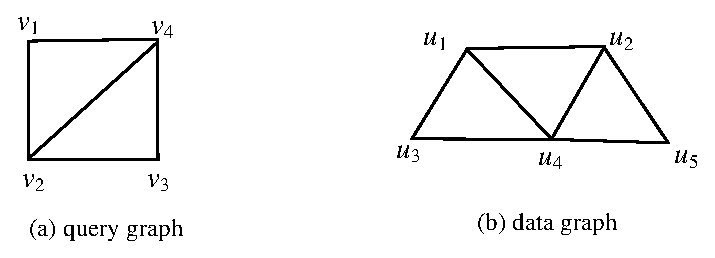
\includegraphics[scale=0.6]{figures/subg.eps}
  \caption{\small{An example of subgraph matching.}}
  \label{fig:subgraph_isomorphism}
\end{figure}

Regarding query vertices as attributes and data vertices as tuples in the relation table, we can naturally express the subgraph join process as joining relations. In \reffig{subgraph_isomorphism}, the edge-by-edge join process can be demonstrated as

\begin{equation}
\label{eq:subgraph_isomorphism}
\small
\begin{aligned}
	R(q) &= R(v_1, v_2) \Join R(v_2, v_3) \Join R(v_3, v_4) \\ 	
	&\Join R(v_4, v_5) \Join R(v_1, v_5) \Join R(v_2, v_5).
\end{aligned}
\end{equation}

\stitle{CliqueJoin.} Generally speaking, the state-of-the-art algorithm \cliquejoin follows the decomposition-and-join framework to do subgraph matching. The main idea of \cliquejoin can be concluded as follows. 

\sstitle{(1) SCP Storage Mechanism.} Considering the SCP storage mechanism for data graph $G$, denoted as $\Phi(G)$, we have $\Phi(G)=\{G_v\ |\ v\in V(G)\}$, $V(G_v)=\{v\} \cup \mathcal{N}(v)$ and $E(G_v)=\{(v,v')\ |\ v'\in \mathcal{N}(v)\}\cup\{(v',v")\ |\ v',v"\in \mathcal{N}(v)\wedge(v',v")\in E(G)\wedge v<v'\wedge v<v"\}$, where $G_v\subseteq G$ is a connected subgraph of $G$ with $v\in V(G_v)$, and $\bigcup_{u\in V(G)}E(G_v)=E(G)$. Each $G_v$ is called the \textit{local graph} of $v$. Suppose the data graph $G$ is maintained in the distributed file system in the form of key-value pairs $(v;G_v)$ for each $v\in V(G)$ according to $\Phi(G)$, a \textit{join unit} is a structure whose matches can be enumerated independently in each local graph $G_v\in \Phi(G)$. For \cliquejoin, the join unit can either be a clique or a star. 

\sstitle{(2) Query Decomposition.} Given a graph storage $\Phi(G)$ and query graph $q$, a query decomposition of $q$ is defined as $D=\{p_0,p_1,\dots,p_t\}$, where each $p_i\in D(0\leq i\leq t)$ is a \textit{join unit} w.r.t. $\Phi(G)$ and $q = \bigcup_{p_i\in D}p_i$. Given the decomposition $D=\{p_0,p_1,\dots,p_t\}$ of $q$, we solve the subgraph enumeration using $t$ rounds of two-way join:

\begin{equation} \label{eq:1}
R(q) = \bowtie_{p_i\in D}R(p_i).
\end{equation}

\sstitle{(3) Optimal Join Plan.} A \textit{join plan} determines an order to solve the above join, which can significantly affect the performance of the algorithm. The join plan is usually presented in a binary tree structure, where the leaf nodes are (the matches of) the join units, the internal nodes are the partial queries. Given a join plan, we compute the join order through a post-order traversal over its binary tree. We denote $P$ as the partial queries set, $P_i$ as the $i$-th partial query whose results are produced in the $i$-th round of the join plan. As a result, a join plan, denoted as $J$, can be uniquely represented as $J = (D, P)$. \cliquejoin utilizes general bushy tree \cite{tree} to represent its join plan. \\

\begin{example}
Figure \ref{fig:tree} shows a join plan for an unlabelled query graph $q$ in the form of a bushy tree. The decomposition of $q$ is $D=\{p_0, p_1, p_2, p_3\}$, and partial query set is $P=\{P_1, P_2, P_3\}$, where $P_3=q$. The first round of join is $P_1 = p_0 \Join p_1$, second round is $P_2=p_2 \Join p_3$, and the final round is $P_3 = P_1 \Join P_2$. In this case, we use triangle ($3$-clique) as the join unit.
\end{example}

\begin{figure}[htb]
  \centering
  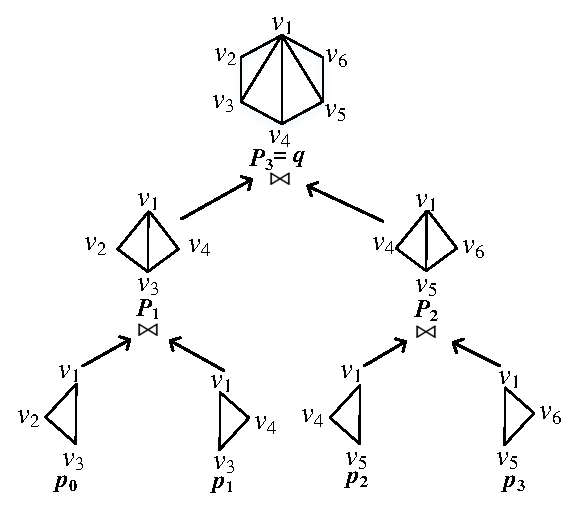
\includegraphics[scale=0.6]{figures/tree.eps}
  \caption{\small{An example of optimal bushy join plan.}}
  \label{fig:tree}
\end{figure}

We denote the set of all possible join plans for query graph $q$ as $\mathcal{S}(q)$. Given a cost function $\mathcal{C}$ defined over $\mathcal{S}$, we say a join plan $\varepsilon$ is \textit{optimal} iff $\mathcal{C}(\varepsilon)$ is minimized. The details of the cost function design can be found in \cite{Lai2016}. However, it is clear that $\mathcal{C}(\varepsilon)$ is positive related to $|R(q)|$.

\sstitle{(4) Matching Result Estimation.} In order to compute the join plan cost  $\mathcal{C}(\varepsilon)$, \cliquejoin needs to estimate $|R(q)|$ for a given query graph $q$. As most of real-life graphs follow \textit{power-law} random distribution\cite{Chung2003}, \cliquejoin estimates $|R_{G_{\text{PR}}}(q)|$ in data graph $G_{\text{PR}}$ generated by power-law model.\\

Considering $q$ is constructed from a single edge by extending one edge at a time in steps. Let $q^{(1)}$ and $q^{(2)}$ be two consecutive queries obtained along the process. More specifically, for some $v\in V(q^{(1)})$ and $v'\in V(q^{(2)})$ such that  $(v,v')\not\in E(q^{(1)})$, $q^{(2)}$ is obtained by adding the edge $(v,v')$ to $q^{1}$. Suppose $f$ is a match of $q^{(1)}$, in principal, we extend $f$ by one more edge to get new matches for $q^{(2)}$. Thus, if the expectation of new matches that can be extended for one certain match of $q^{(1)}$ is $\lambda$, we have:
\begin{equation} \label{eq:r}
|R_{G_{\text{PR}}}(q^{(2)})|=\lambda |R_{G_{\text{PR}}}(q^{(1)})|
\end{equation}

The value of $\lambda$ depends on the edge which extends $q^{(1)}$ to $q^{(2)}$. There are two cases may happen, that is, $v'\not\in V(q^{(1)})$ and $v'\in V(q^{(1)})$. The details of the two cases for computing $\lambda$ and the algorithm of computing $|R_{G_{\text{PR}}}(q)|$ by extending edges can be found in \cite{Lai2016}.

\stitle{Timely Dataflow.} \timely dataflow system is a high performance distributed system. It abstracts the computation model as a dataflow graph. The node in the dataflow graph is responsible for doing computations and the edge is to send data streams to nodes. One node can receive several input streams and produce one output stream. When the dataflow graph for the given computation task is constructed, it will distribute data to each worker in the cluster, and each worker can finish its computation locally. The whole computation task is finished when there is no output stream produced by workers.

\section{Optimizations}
\label{sec:opt}

\cliquejoin is proposed for unlabelled graphs and implemented on MapReduce. In this section, we introduce \gencliqjoin, our revision of \cliquejoin to extend the algorithm to labelled graphs and dataflow model.

\subsection{Cost Analysis for Labelled Matching}

We can use the label information in the graph to refine the result size estimation strategy in \gencliqjoin. Intuitively, we should process query graphs with rare labels as fast as possible to reduce the cost. \\

We use $\Pr_{G}(\iota)$ to denote the probability of the label $\iota$ that appears in a certain node of data graph $G$. Then, \eqref{eq:r} can be refined as:
\begin{equation} \label{eq:rr}
|R_{G}(q^{(2)})|=\eta\lambda |R_{G}(q^{(1)})|
\end{equation}

Similarly, the value of $\eta$ is considered in two cases:

\begin{itemize}
\item \textbf{(Case 1)} If $v'\not\in V(q^{(1)})$, a new vertex is introduced in $q^{(2)}$ as well as a new edge. In this case, we have:
\begin{equation} \label{eq6-new}
 \textstyle \eta = \Pr_{G}(L(v')) \times \Pr_{G}(L((v,v')))
\end{equation}

\item \textbf{(Case 2)} If $v'\in V(q^{(1)})$, an edge is added between two existing vertices in $q^{(1)}$. In this case, we have:
\begin{equation} \label{eq:7-new}
\textstyle \eta = \Pr_{G}(L((v,v')))
\end{equation}
\end{itemize}

In addition, $\Pr_{G} (\iota)$ can be calculated using the maximum likelihood estimation via sampling or scanning the data graph $G$.

\subsection{Migration from MapReduce to Dataflow} \label{to-df}

\stitle{Implementation Details.}  The SCP storage mechanism and optimal join plan generation for unlabelled querie are strictly implemented according to \cite{Lai2016}. For labelled queries, we firstly scan the data graph to acquire label frequencies and apply the optimized cost model we propose in Section \ref{sec:opt} afterward. Here, given a join plan $J$, we will show the details of how to implement \gencliqjoin on \timely dataflow next. 

\sstitle{(1) Building \timely Dataflow.} The procedure of building the dataflow is shown in Algorithm \ref{alg:build_dataflow}. This algorithm is to compute the join operations round by round to get the final matches $R(q)$ in a stream.\\

There are two inputs of the algorithm: an $InputHandle$ set $I$ and a join plan $J$. An $InputHandle$ is a handler in \timely to store data. The data in $InputHandle$ can be converted to stream directly by invoking $to\_stream$ operation in \timely. We use $I$ to store all join unit's matches $R(p_i)$, where $p_i \in D$. Join plan $J$ consists of $|J|$ rounds of join configurations. One round configuration $j\in J$ includes left subgraph, denoted as $j.lg$, right subgraph, denoted as $j.rg$, join key, denoted as $j.join\_key$, and batch parameters, denoted as $j.batch\_params$. With the configurations in $j$, we know exactly what we should do in each round of join. \\

In line 1-2, if there is only one element in $I$, it means the query graph $q$ is a join unit, and we don't need to do join operations. Therefore, we just return the streaming result of $I[0]$. In line 3, for the join order is consistent with post-order traversal over the binary tree (e.g. Figure \ref{fig:tree}), we use a stack \textit{StreamStack} to store $R(P_i)$, where $P_i$ is a partial query. In line 5, for each join $j$ in $J$, we first find its left and right subgraph matches in stream, denoted as $LStream, RStream$ (line 6), respectively. In line 6-16, we consider two cases: (1) If the left/right subgraph is a join unit, we simply fetch its stream in $I$. (2) If left/right subgraph is a partial query, we can get its stream by popping the top element in $StreamStack$. Then we use \code{BatchJoin} to join $LStream$ and $RStream$ under the configuration $j$ (line 17), and push the result stream $RstStream$ onto $StreamStack$ (line 18). When we complete the iteration over $J$, we pop the top element as the final result stream, which is $R(q)$.

\begin{algorithm}[htb]
\SetAlgoVlined
\SetFuncSty{textsf}
\SetArgSty{textsf}
\small
\caption{\code{BuildDataflow}($InputHandle$ set $I$, join plan $J$)}
\label{alg:build_dataflow}
\If{$|I| = 1$} {
\State{\textbf{Return} $I[0].to\_stream()$;}
}
\State{$StreamStack \leftarrow \emptyset$;}\\
\State{$i \leftarrow 0$;}\\
\ForAll{$j \in J$}{
    \State{$LStream \leftarrow \emptyset;$}
    \State{$RStream \leftarrow \emptyset;$}\\
    \If{$j.lg$ is a join unit}{
        \State{$LStream \leftarrow I[i].to\_stream()$;}\\
        \State{$i \leftarrow i + 1$;}
    }
    \Else{
        \State{$LStream \leftarrow StreamStack.pop()$;}
    }
    \If{$j.rg$ is a join unit}{
        \State{$RStream \leftarrow I[i].to\_stream()$;}\\
        \State{$i \leftarrow i + 1$;}
    }
    \Else{
    \State{$RStream \leftarrow StreamStack.pop()$;}
    }
    \State{$RstStream \leftarrow  \code{BatchJoin}(LStream, RStream, j)$;}\\
    \State{$StreamStack.Push(RstStream)$;}
}
\State{\textbf{Return} $StreamStack.pop()$;}
\end{algorithm}


\sstitle{(2) Computing Join Unit Matches.} Before we run Algorithm \ref{alg:build_dataflow}, we need to precompute all join unit matches $R(p_i)$, where $p_i \in D$. The process of computing $R(p_i)$ is illustrated in Algorithm \ref{alg:join_unit_comp}. The inputs of the algorithm include join plan $J$ and the local data graph $G$. In line 1, we initialize \textit{InputHandle} set $I$ with length $|J.D|$, which is exactly the number of join units in $J$. In line 3-11, for each join $j\in J$, if left/right subgraph $j.lg/j.rg$ is a join unit, we compute its matches $R_G(j.lg)/R_G(j.rg)$ in local graph $G$ and send them to the corresponding input handler $I[i]$, where $p_i$ is the $i$-th join unit in $J$. In line 12, we return the join unit matches $I$. 


\begin{algorithm}[htb]
\SetAlgoVlined
\SetFuncSty{textsf}
\SetArgSty{textsf}
\small
\caption{\code{CompUnitMatches}(join plan configuration set $J$, local data graph $G$)}
\label{alg:join_unit_comp}
\State{$I \leftarrow$ new $InputHandle$ set with size of $|J.D|$;}\\
\State{$i \leftarrow 0$;}\\
\ForAll{$j \in J$}{
    \If{$j.lg$ is a join unit}{
        \State{$M \leftarrow R_{G}(j.lg)$;}\\
        \State{send $M$ to $I[i]$;}\\
        \State{$i \leftarrow i + 1$;}
    }
     \If{$j.rg$ is a join unit}{
        \State{$M \leftarrow R_{G}(j.rg)$;}\\
        \State{send $M$ to $I[i]$;}\\
        \State{$i \leftarrow i + 1$;}
    }
}
\State{\textbf{Return} $I$;}
\end{algorithm}


\sstitle{(3) Joining Two Streams in Batch.} We observe that when directly implementing join of two streams, the huge intermediate results on large data graph will very likely consume the memory up. Therefore, we implement the external hash join following \textit{buffer-and-batch} idea to save memory, which is shown in Algorithm \ref{alg:batch_join}. The inputs of the algorithm are two streams $S_1, S_2$ and the join configuration $j$. In line 1-2, we buffer the data in $S_1/S_2$ to $B_1/B_2$. More specifically, we buffer the data from stream to a given threshold configured in $j.batch\_params$, and sort it according to $j.join\_key$ before spilling to the disk. In line 3-7, while the buffered data $B_1/B_2$ is not empty, we read the data from disk to $buffer_1/buffer_2$ batch by batch (line 4-5). Then we join $buffer_1$ and $buffer_2$ according to the join key in $j$, and output the result (line 6-7). In this way, the memory consumed by each join is one batch of data and we can configure the batch size in $j.batch\_params$ according to the machine's memory capacity. 


\begin{algorithm}[htb]
\SetAlgoVlined
\SetFuncSty{textsf}
\SetArgSty{textsf}
\small
\caption{\code{BatchJoin}(left stream $S_1$, right stream $S_2$, join configuration $j$)}
\label{alg:batch_join}
\State{$B_1 \leftarrow S_1.buffer(j)$;}\\
\State{$B_2 \leftarrow S_2.buffer(j)$;}\\
\While{$B_1 \not= \emptyset$ and $B_2 \not= \emptyset$ }{
    \State{$buffer_1 \leftarrow B_1.next\_batch()$;}\\
    \State{$buffer_2 \leftarrow B_2.next\_batch()$;}\\
    \State{$result \leftarrow buffer_1 \Join buffer_2$ according to $j.join\_key$;}\\
    \State{\textbf{Output} $result$;}
}
\end{algorithm}

\section{Experiments}
\label{sec:exp}
In this section, we conduct extensive experiments for \gencliqjoin on both unlabelled and labelled data graphs. Here, we only consider undirected graph matching because an undirected edge can be regarded as two directed edges. We will show the experimental results over the optimizations we have done to \cliquejoin.
\subsection{Experimental Settings}
\stitle{Environments.} We use a cluster of 10 nodes connected via a 10Gpbs switch, and each node has 64GB memory, 1TB disk and 1 Intel Xeon CPU E3-1220 V6 3.00GHz with 4 physical cores. We implement \cliquejoin in \timely dataflow system \footnote{\url{https://github.com/frankmcsherry/timely-dataflow}} using Rust 1.27. We use 10 machines and each machine uses 3 workers by default.

\stitle{Metrics.} We measure query time $T$ from the average time of three runs. The query time is actually the slowest worker's running time during each run, which excludes graph loading time as it is negligible compared to query time. We set batch size to 10,000 and threshold to 10,000,000 by default in $\code{BatchJoin}$.

\stitle{Preprocessing Datasets.} We preprocess each dataset as follows: we treat it as a simple undirected graph by removing self-loop and duplicate edges, and reorder the node id according to the degree and represent it using Compressed Sparse Raw (CSR)\footnote{\url{https://en.wikipedia.org/wiki/Sparse_matrix}}.

\subsection{Unlabelled Matching}
\label{sec:unlabelled_matching}
\stitle{Datasets.} We evaluate 3 real graphs of different sizes and types. The sources of these graphs are from Snap\footnote{\url{http://snap.stanford.edu/data/index.html}} and WebG\footnote{\url{http://law.di.unimi.it/datasets.php}}. We consider the following two graph types: Social Network (Soc) and Web Graph (Web).  We list the evaluated graphs in \reftable{unl_datasets}. Note that both $|V(G)|$ and $|E(G)|$ are in millions. 

\begin{table}
\centering
 \begin{tabular}{|c|c|c|c|c|c|c|} 
 \hline
 Datasets & Name & $|V(G)|/mil$ & $|E(G)|/mil$ & $\overline{d(G)}$ & $D(G)$ \Ts\Bs \\
 \hline\hline
 livejournal & LJ & 4.85 & 43.37 & 8.9 & 20,333  \\
  \hline
 orkut & OK & 3.07 & 117.19 & 38.1 & 33,313 \\
 \hline
uk2002 & UK & 18.5 & 298.11 & 16.1 & 194,955\\
\hline
 \end{tabular}
\caption{The Unlabelled Datasets.}
\label{tab:unl_datasets}
\end{table}

\stitle{Queries.} The five queries denoted by $q_1$ to $q_5$ are illustrated in \reffig{unlq}, where the number of nodes vary from 4 to 5 and the number of edges vary from 4 to 10. We assign the order of the nodes for symmetry breaking\cite{Grochow2007} under each query graph. Here, we have considered all queries for fair comparisons.

\begin{figure}[htb]
  \centering
  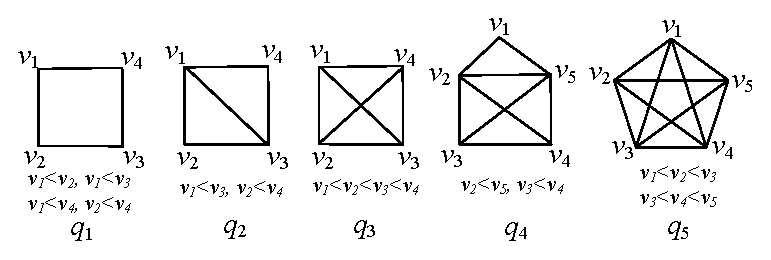
\includegraphics[scale=0.6]{figures/unlq.eps}
  \caption{\small{Unlabelled Queries.}}
  \label{fig:unlq}
\end{figure}

\stitle{Exp1 - Vary Queries.} We compare \gencliqjoin with \cliquejoin by testing all queries on LJ, which is shown in \reffig{vary_query}.Note that for better presentation, the ordinate is calculated by $logT$, where $T$ is the query time. We can see that for enumerating the join unit $q_3$(4-clique) and $q_5$(5-clique), \gencliqjoin outperforms \cliquejoin by more than one order of magnitude. For $q_2$, \gencliqjoin is 2 times faster than \cliquejoin. However, \cliquejoin outperforms \gencliqjoin in $q_1$ and $q_5$. TODO: Explain them.

\begin{figure}[htb]
  \centering
  \includegraphics[scale=0.4]{figures/exp1.pdf}
  \caption{\small{Vary Queries.}}
  \label{fig:vary_query}
\end{figure}

\stitle{Exp2 - Vary Datasets.} We compare \gencliqjoin with \cliquejoin by querying $q_2$ and $q_5$ on all datasets in order to show the good performance over different data properties. The results are shown in \reffig{vary_dataset}. We can see that, when querying $q_2$, \gencliqjoin generally outperforms \cliquejoin by around 2 times. When querying $q_5$, \gencliqjoin is 3 to 10 times faster than \cliquejoin. 

\begin{figure}[htb]
  \flushleft
  \includegraphics[scale=0.3]{figures/exp2.pdf}
  \caption{\small{Vary Datasets.}}
  \label{fig:vary_dataset}
\end{figure}


\stitle{Exp3 - Scalability.} We compare the scalability of \gencliqjoin with \cliquejoin on LJ using $q_2$ by varying number of nodes(6, 8, 10) used in the cluster, whose results are shown in \reffig{unl_sca}. We can see that \gencliqjoin is in general 2 times faster than \cliquejoin.

\begin{figure}[htb]
  \centering
  \includegraphics[scale=0.37]{figures/exp3.pdf}
  \caption{\small{Unlabelled Scalability.}}
  \label{fig:unl_sca}
\end{figure}


\subsection{Labelled Matching.} We use LDBC social network benchmarking (SNB)\cite{Ldbc} for labelled matching experiment for the lack of big public labelled graphs. SNB provides a data generator that can generate synthetic social networks of statistics, and a document\cite{LdbcDoc} that describes the benchmarking tasks, which are actually doing subgraph matching. To the best of our knowledge, there are few experiments of distributed labelled subgraph matching on large datasets. Therefore, in this section, we will just demonstrate the effectiveness and scalability of \gencliqjoin when doing labelled subgraph matching.

\stitle{Datasets.} We list the datasets and their statistics in \reftable{l_datasets}. All datasets are generated using the "Facebook" mode with a span of 3 years. The dataset's name, denoted as DG$x$, represents a scale factor of $x$. As mentioned before, we first parse the graph into undirected simple graph. Then we remove all properties except the node types as labels, and the label is encoded as an integer to accelerate the matching.

\begin{table}
\centering
 \begin{tabular}{|c|c|c|c|c|c|c|} 
 \hline
 Name & $|V(G)|/mil$ & $|E(G)|/mil$ & $\overline{d(G)}$  & $D(G)$ & \#Labels \Ts\Bs \\
 \hline\hline
 DG01 & 3.2 & 17.24 & 10.84 & 464,368  & 11 \\
  \hline
 DG03 & 9.28 & 52.65 & 11.3 & 1,346,287 & 11 \\
 \hline
 DG10 & 29.99 & 176.48 & 11.77 & 4,282,812 & 11 \\
\hline
 DG30 & 88.79 & 540.51 & 12.17 &  12,684,488 & 11 \\
\hline
 DG60 & 187.11 & 1246.66 & 13.32 & 26,639,563 & 11 \\
\hline
 \end{tabular}
\caption{The Labelled Datasets.}
\label{tab:l_datasets}
\end{table}

\stitle{Queries.} The labelled queries are shown in \reffig{lq}, which are generated from SNB's tasks with following rules: (1) removing the direction of edges and edge labels; (2) using one-hop edge for multi-hop edges; (3) removing the "no edge" and unconnected graph condition; (4) removing all properties except the node type as its label. For (1), we do the adaptation for simplicity although we can support that case. We adapt (2) and (3) for consistency with the subgraph matching problem studied in this paper. We adapt (4) for our implementation currently can not support property graphs.

\begin{figure}[htb]
  \centering
  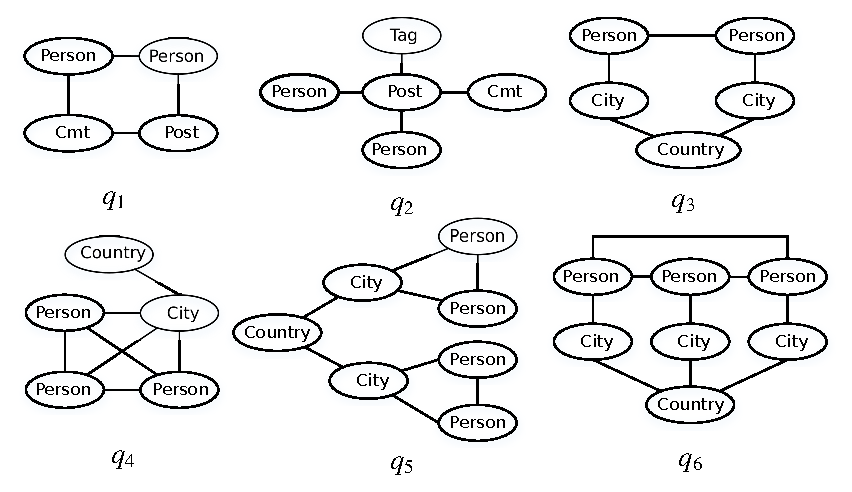
\includegraphics[scale=0.6]{figures/lq.eps}
  \caption{\small{Labelled Queries.}}
  \label{fig:lq}
\end{figure}

\stitle{Exp4 - All Labelled Queries.} We perform \gencliqjoin for all queries on all datasets, and the results are illustrated in \reffig{all_lq}(whose ordinate is the logarithm of query time $T$). We can see that \gencliqjoin can finish subgraph matching in tens of seconds for $q_2, q_3, q_4, q_5, q_6$ in all data graphs, even if DG60 is a billion scale graph. We notice that the query time for $q_1$ increases sharply when the dataset becomes larger. The reason is that the algorithm spends a lot of time computing the stars' matches in $q_1$($q_1$ is decomposed to two 2-star(s)) due to the poor filter information of $q_1$'s join units in data graph.

\begin{figure}[htb]
  \centering
  \includegraphics[scale=0.4]{figures/exp4.pdf}
  \caption{\small{All Labelled Queries.}}
  \label{fig:all_lq}
\end{figure}

\stitle{Exp5 - Labelled Scalability.} We evaluate the labelled matching scalability of $q_1$ and $q_4$ on DG10 by varying the number of nodes used in the cluster(6, 8, 10), and the results are demonstrated in \reffig{l_sca}. We can see that when decreasing the number of machines used in the cluster, the query time slightly increases, which shows that \gencliqjoin has great scalability for labelled matching.

\begin{figure}[htb]
  \centering
  \includegraphics[scale=0.4]{figures/exp5.pdf}
  \caption{\small{Labelled Scalability.}}
  \label{fig:l_sca}
\end{figure}


\section{Realted Work}
\label{sec:rel}

\stitle{Subgraph Enumeration.}  Besides the sequential algorithms we have mentioned in Section \ref{sec:intro}, GraphQL \cite{graph-ql} and SPath \cite{spath} focus on reducing the candidates of query vertices by exploiting neighborhood-based filtering. \turboiso \cite{turbo-iso} and the boost technique in \cite{subgraph-boost} propose to merge vertices with same labels and the same neighbours in $q$ and $G$ respectively to reduce the matching complexity. \cite{comparison} provides an in-depth comparison of above mentioned subgraph isomorphism algorithms. A more recent work in \cite{bi-fei} uses a data structure called \textit{compact path index} (CPI) to store the potential embeddings of a spanning tree of the query graph to improve both time and space efficiency. Algorithms of subgraph enumeration mainly focuses on answering a single query, \cite{multi-query} studied the problem of \textit{multiple query optimization} (MQO) for subgraph enumeration. The details of distributed subgraph enumeration algorithms can be found in Section \ref{sec:intro}.

\stitle{Subgraph Containment Search.} Let $\mathcal{D}=\{g_1,g_2,\dots,g_N\}$ be a graph database that has $N$ graphs, the problem of subgraph containment search over a graph database is to identify if the graphs in $\mathcal{D}$ contain the given query graph $q$. To speed up the search, many graph-feature based approaches have been proposed, performing graph indexing and adopting a filter-and-verification framework. As a result of such approach, false positives are removed by a pruning strategy before subgraph isomorphism algorithm is performed on each of the remaining candidates to obtain the final results. Existing works includes \textit{frequent subgraph mining based approaches} (e.g., gIndex \cite{gindex}, Tree+$\Delta$ \cite{tree+}, and FG-Index \cite{fg-index}) and \textit{exhaustive enumeration based approaches} (e.g., gCode \cite{gcode}, CT-Index \cite{ct-index}, GraphGrep \cite{graph-grep}, GraphGrepSX \cite{graph-grep-sx}, Closure-tree \cite{closure-tree}, and Grapes \cite{grapes}). In approximate graph containment search, TALE \cite{tale} was proposed.

\section{Concolusion}
\label{sec:conclusion}
In this paper, we study the distributed subgraph matching algorithm \cliquejoin. Discovering the limitations of \cliquejoin that can not handle labelled subgraph matching, we propose \gencliqjoin to generalize it by extending its cost evaluation function to labelled graphs so that it can generate optimal join plan for labelled query graphs. We further improve its performance by migrating \cliquejoin from Map-Reduce to \timely dataflow system, which can significantly reduce the I/O cost. We conduct extensive experiments on both unlabelled and labelled matching. The experimental results show that the generality and performance of \cliquejoin are highly improved after performing the two optimizations we propose in this paper.

\bibliographystyle{abbrv}
\bibliography{icde}

\end{document}